\section{Event structures}
\label{sec:event-structures}
    Event structures were developed in \cite{winskel80events} as an attempt to bridge Petri net theory\footnote{Petri nets are considered a classical model of concurrency with important ideas to understand the current research. Research into Petri nets has been done extensively in models of concurrency literature. Hence, we will not investigate Petri nets. One can find an introduction to Petri nets in \cite{Petri73petrinets}, and one can also find a recent comparison to modern models of concurrency in \cite{Goubault18RelationshipsModelsForConcurrency}.} and domain theory. Specifically, event structures is considered an extension to stable families, which are sets of all events which may have occurred by some stage, or history, in the evolution of a process. An event structure represents a process. We will adopt the same notion as used by Winskel \cite{NielsenPW81eventstructures} and Van Glabbeek $\&$ Goltz \cite{GlabbeekP09configStruct} that families are called \emph{configuration structures}. This bridge between Petri nets and domain theory would allow concurrent systems to be translated into automata, or schedules, providing a schedule-automata duality \cite{NielsenPW81eventstructures, GlabbeekP09configStruct}.
    
    %Event structure were developed in \cite{winskel80events} as an attempt to bridge Petri net theory and domain theory. In a Petri net, the state is given by a marking, but the same marking can be reached after several different sets of transitions. Thus the information theoretic content of a marking is rather obscure. Event structures remedy this by making the state of a system be exactly the set of actions that have occurred so far. However in Petri net multiple occurrences of the same action can occur, so if a state just recorded which actions had occurred and some actions occurred many times, this information would be forgotten. But since the purpose of a state is to keep as much information as possible, the concept of event or occurrence of an action was introduced. An event is an action which occurs at most once in an execution. In this thesis, we will not investigate into Petri nets, however, one can find an introduction to Petri nets in \cite{Petri73petrinets}.
    
%    Event structures describe a concurrent system through the occurrence of events, like "send message" and "fetch message". This is done through a partial ordering $\leq$ on the set of events $E$. The formal definition is as follows

 \begin{definition}[Event structure \cite{winskel95modelsCategory}]\label{def:event-structure}
    An event structure ($E, \leq, \#$) consists of a set $E$, of events which are partially ordered by $\leq$ (the causal dependency relation) and a binary, symmetric, irreflexive relation $\# \subseteq E \times E$ (the conflict relation) which satisfy
    
    \begin{itemize}
        \item $\{ e'\ |\ e' \leq e\}$ is finite (axiom of \emph{finite causes}), and
        \item $e \# e'$ and $ e' \leq e'' \Rightarrow e \# e''$ (conflict is \emph{hereditary}).
    \end{itemize}
    
    for all $e, e', e'' \in E$.
\end{definition}

Event structure is formally defined as a triple ($E, \#, \leq$), where $E$ is the set of events, $\# \subseteq E \times E$ is a conflict relation, and $\leq\ \subseteq E \times E$ is a partial order. If two events are in conflict, not both of them can happen in a single execution. Also, for the event $e$ to happen, all the events before it in the partial order must have happened. We consider that events $e$ and $e'$ are \emph{concurrent}, denoted $e\ co\ e'$, as follows:

    \begin{center}
        $e\ co\ e'\ $ iff $not\ ((e \leq e')$ or $(e' \leq e)$ or $e \# e'))$.
    \end{center}

If $e$ and $e'$ are not dependent on each other in either order and there is no conflict, then we may run $e$ and $e'$ concurrently.

The events in a prime event structure can be thought of as event occurrences without significant duration, in any history an event appear at most once. The relation of \emph{immediate} dependency $e \rightarrow e'$ means $e$ and $e'$ are distinct with $e \leq e'$ and also that there is no event in between.

 \begin{definition}[Configurations \cite{winskel95modelsCategory}]\label{def:configurations-event-structure}
    Let ($E, \leq, \#$) be an event structure, and its \emph{configurations}, $\mathcal{D}(E, \leq, \#)$, to consist of those subsets $x \subseteq E$ which are
    
    \begin{itemize}
        \item conflict-free: $\forall e, e' \in x . \neg (e \# e') and$
        \item downwards-closed: $\forall e, e' . e' \leq e \in x \Rightarrow e' \in x$.
    \end{itemize}
\end{definition}

As shown by Winskel in \cite[Proposition 18]{winskel95modelsCategory}, we can recover the important relations, such as conflict and partial order, associated with an event structure from its finite configurations. We will not present that here. We will, however, use configurations in our definition of a category of event structures. First, we have to introduce morphisms of event structures.

 \begin{definition}[Morphisms of event-structures \cite{winskel95modelsCategory}]\label{def:morphisms-event-structure}
    Let $ES$ = ($E, \leq, \#$) and $ES'$ = ($E', \leq', \#'$) be event structures. A \emph{morphism} from $ES$ to $ES'$ consists of a partial function $\eta : E \rightarrow_{*} E'$ on events which satisfies
    
    \begin{itemize}
        \item $x \in \mathcal{D}(ES) \Rightarrow \eta x \in \mathcal{D}(ES')$,
        \item $\forall e, e' \in x . \eta (e), \eta (e')$ are both defined, and
        \item $\forall e, e' \in x . \eta (e) = \eta (e') \Rightarrow e = e'$.
    \end{itemize}
\end{definition}

If we let ($E, \leq, \#$) be an event structure and let $x, x'$ be configurations, then we write $x \xrightarrow{e} x' \Leftrightarrow e \notin x$ and $x' = x \cup \{e\}$. From Proposition 19 in \cite{winskel95modelsCategory}, we have that two events $e$ and $e'$ are concurrent if and only if there exists configurations $x_1, x_2, x_3$ and $x_4$ such that we get the interleaving square, as shown in Figure \ref{fig:interleaving-square-event-structure}.

\begin{figure}[ht]
        \centering
        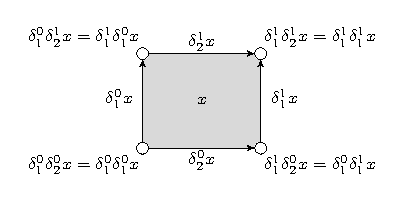
\includegraphics[scale=1.3]{Figures/2.Models-for-concurrency/event-structure/interleaving-square.pdf}
        \captionof{figure}[Configurations of an event structure]{An event structure with two concurrent events $e$ and $e'$ such that we get the configurations $x_{1}, x_{2}, x_{3}$, and $x_{4}$. The configurations generate the interleaving square because of the way the concurrent events $e$ and $e'$ form a square.}
        \label{fig:interleaving-square-event-structure}
\end{figure}



 We write $\allES$ for the category of event structures. Also, we name $\allES_{E}$ its subcategory where we restrict to event structures labeled on an alphabet $E$. The alphabet $E$ can be considered the same as the set of events $E$. Events are considered one side of a duality \cite{Pratt02eventStateDuality}, where automata is the other side. In Section \ref{sec:Chu-spaces} we will introduce Chu spaces \cite{gupta94phd_Chu}, which is a general framework where automata and schedules, with the Chu duality, can be converted into one another. Both automata and schedules have applications in different fields of computer science such as hardware design and analysis of asynchronous circuits, network diagnostics, distributed computation and logics of programs. 